\documentclass[a4paper,twoside]{article}
\usepackage{graphicx}                                     
\usepackage{adjustbox}   
\usepackage{epsfig}
\usepackage{subcaption}
\usepackage{calc}
\usepackage{amssymb}
\usepackage{amstext}
\usepackage{amsmath}
\usepackage{amsthm}
\usepackage{multicol}
\usepackage{pslatex}
\usepackage{apalike}
\usepackage{SCITEPRESS}     % Please add other packages that you may need BEFORE the SCITEPRESS.sty package.


\begin{document}

\title{Visual-inertial sensor fusion via machine learning}

\author{\authorname{Habib Boloorchi\sup{1}\orcidAuthor{0000-0000-0000-0000}, He Bai\sup{1}\orcidAuthor{0000-0000-0000-0000} and Christopher Crick\sup{2}\orcidAuthor{0000-0000-0000-0000}}
\affiliation{\sup{1}Department of Computer Science, Oklahoma State University, My Street, MyTown, MyCountry}
\affiliation{\sup{2}Department of Computing, Main University, MySecondTown, MyCountry}
\email{\{f\_author, s\_author\}@ips.xyz.edu, t\_author@dc.mu.edu}
}

\keywords{The paper must have at least one keyword. The text must be set to 9-point font size and without the use of bold or italic font style. For more than one keyword, please use a comma as a separator. Keywords must be titlecased.}

\abstract{Robot localization is a well-studied problem, with many competing solutions, from odometry to inertial measurement to SLAM to GPS and other beacon-based approaches. Some methods work only with certain modalities: measurement of wheel odometry is useless for legged or flying locomotion, for instance. Visual landmark detection and dead reckoning are useful to robots with many different structures and means of locomotion, and can be implemented with very low-cost cameras and inertial measurement units (IMUs). However, existing approaches require fairly sophisticated hardware with precise, rapid, real-time control loops in order to fuse the visual inertial odometry data adequately. We present algorithms to better handle the uncertainty which stems from noisy, inconsistent IMU and machine vision data, using a machine learning approach to provide a robot better awareness of its location and the effect of its self-motion on visual cues. This approach yields robust localization performance which generalizes across very different robot platforms using low-cost sensing and computation.}

\onecolumn \maketitle \normalsize \setcounter{footnote}{0} \vfill

\section{\uppercase{Introduction}}
\label{sec:introduction}

Data fusion  in Robotics has a huge and wide spectral of fields. The aim of most scientists in this area is helping robots to be more autonomous than before. One of the puzzles in this area is Navigation and localization is its bottleneck because a robot needs to have an estimation its state. In other words, having consciousness on where it is, will be a must for decision on next steps .
In our research, we found flexibility in data fusion for the process of localization baffling.Not only, Concise timing is matter but we also found lack of a Software that help us handle devices that can do localization which does not required expert, cost and energy. This necessity to consistency and having experienced in mechanical and electronic engineers and an expensive device lead us to create a device that can work better with less consistency in data fusion.
The demand to having data fusion stems from the role of Visual-inertial odometry. Visual-inertial odometry needs to gather data from both perception and Inertial Measurement Unit(IMU). This Odometry can estimate Coordinate in 3 Dimensional world,which Opticounters and GPS can only do it in 2 Dimension, when corresponding data is received in a consistent latency.   


The Perceptio part is added to inertial odometry to be more Robust to uncertainty. Vision of localization can handle the situation in a variety of environments such as GPS unfriendly places and inertial can overcome situations such as dark or low textured, which could not let the camera has good perception.
These challenges shows up when we use visual inertial odometry:
\begin{itemize}
\item Combining data that comes from IMU and camera should offer the least latency and be so accurate. and if not algorithms could not work well.
\item Even if we could create a device that works accurately calibration each time we use it in order to have good results would cost so much time.
\item Cost of stable Visual inertial odometry sensor is so high
\item Most of the Visual inertial Odometry applications are not enough user-friendly for calibration and regular use. you need to be an expert in Control to know the terms.
\end{itemize}
In order to have more sense of these deficiencies, we can come up with an example. In Agriculture Departments, we have a big population of plants that we need to know the effect of each variable on plants. These kinds of research need to observe every plant and this can be tested by taking Photo of each plant. Visual inertial odometry can help us to localize a self-announcement mobile vehicle that can pull the trigger of shutter. Now it comes more baffling when we need an expert in control who is also a scientist in agriculture. 
We offered a machine learning approach that can resolve the combining data, expenses, and requirement of an expert.
We get data to do the preprocessing that does not need the information of the camera or cameras for the perception. It can work with every visual-inertial sensors. These sensors can be cheap because the learning procedure is robust to noises.
In our method we does perception using essential matrix then we take advantage of Random Forest Regression method to estimate the Position of the robot.  

 
 
 
\section{\uppercase{Related Works}}
When it comes to reduce the uncertainty, localization has a vital role \cite{cadena2016past}. 
In other words, Odometry is using motion data comes from sensors in order to reduce the uncertainty of robots position in environment\cite{huang2017visual,valencia2018mapping}.This data can come from rotation of wheels, GPS, IMU(Inertial Measurement Units), Cameras.
In large-scale Domains GPS (Global Positioning System) is one of the most popular for localization but it has some draw backs in smaller space. For example it does not have enough accuracy and also there is some places it is not feasible to use it. For instance, under water, as a GPS-denied circumstance, we can realize that we need a robocentric approach for other ways for odometry \cite{saska2017system}.
IMU(Inertial Measurement Units) is one of the tools that can be helpful in approximation of the trajectory \cite{gui2015mems}. However, when we use IMU some problems as a matter of noisy data and motor noises on devices can be appeared. Furthermore, we need to have trajectory in circumstances as an example Mars Rovers specifically we cannot use it alone.\cite{mars-rover-slam}  
Rotary encoders that can estimate wheels rotation with getting pulse from opto-counters is a technique for wheeled robots while this instrument cannot be useful for highly dynamic cases such as bipedal robots or in three dimensional spaces for flying robots.  \cite{rovio15}.
The human inspired visual ego-motion can be counted as a liable approach to extract trajectory\cite{engel2018direct}. This Motion estimation, which apply machine vision, is called Visual Odometry. One of the most application of Visual Odometry is SLAM (Simultaneous Localization and Mapping) \cite{orb-slam1,orb-slam2,forster2017svo,mueggler2017event}.
One of the problems that ORB-SLAM1\cite{orb-slam1} ,as an example of best Visual Odometry shows is drifting stems from lack of having closed loop algorithms.\cite{7817784}. Another, disadvantage that can lead to get lost as a robot is having fast angular movements that can lead to miss of landmarks. Since these landmarks are critical sources to estimate the position of our path, robot can lose its position. Thus, vision need to be aided by IMU. In addition, the integration of IMU can offers some benefits\cite{leutenegger2015keyframe}. accuracy can be named as one of these advantages\cite{rovio17,schneider2018maplab,sun2018robust}. 

We can integrate images and Inertial data via variety of algorithms. Using probability to estimate the better likelihood of location\cite{bowman2017probabilistic} is one of the approaches to estimate the position. However, It is more popular to do this fusion can be done by extended Kalman filter\cite{lynen2013robust}. The advantage of Extended Kalman Filter and Uncented Kalman Filter from Kalman filter is using Jacobian to extract the position of the robot in nonlinear system \cite{julier2004unscented,wan2000unscented}.

 The major difference between UKF and EKF is their ability to estimate in the nonlinear system. In other words EKF is more for weak nonlinearity system while UKF is for high nonlinearity system. \cite{st2004comparison}
 
Bloesch et al \cite{rovio15,rovio17}mars-rover-slam  offers Iterated Extended Kalman Filter in order to robust the ability of estimation of trajectory. Iterations can robust the ability to find the maximum likelihood to estimate the position of a robot by robocentric formula \cite{rovio15,rovio17}. 


To do landmark detection, Bloesch et al.  employed Shi-Tomasi algorithm \cite{shi1993good}. In this method, landmarks is extracted by utilization of three times down sampling and more probable landmarks between candidates will be chosen. ROVIO (Robust Visual Inertial odometry) uses these landmarks and by warping of land marks the movement in perception can be estimated.

Other innovations can conceive the ego-motion \cite{zhou2017unsupervised} using unsupervised learning. To understand the motion. This algorithm uses Convolutional Neural Network to find out the warping. As we have three dimensional views using RGB-d or Stereo cameras we can both interpret angular and linear movements.

Although, There are several datasets that contains ground truth in 6 degree of freedom that shows angles and also position of the a flying robot and a get data from inertial sensors and stereo cameras\cite{euroc},in this article, we want to make sure that we process data real-time and we also want to use our algorithm on flying robots. so we suggested a creation of device that able to get inertial and perception data relatively. we also suggested a creation of anew device to collect a data to have relative image and IMU data and having less delay with getting th data.

 our perception is based on the aforementioned Rovio \cite{rovio17}, and integrate it to IMU data.  Instead of using iterated Extended Kalman Filter, we are going to take advantage of supervised Learning  to create trajectory.
 Although, our method cannot show the result as accurately as Rovio, we offer benefit of having more robustness to latency inconsistency in devices such as the one show in Figure \ref{fig:vio} which has received in a progress without pattern that we see in Figure \ref{fig:incons}. 
 




\begin{figure}[!h]
  \centering
   {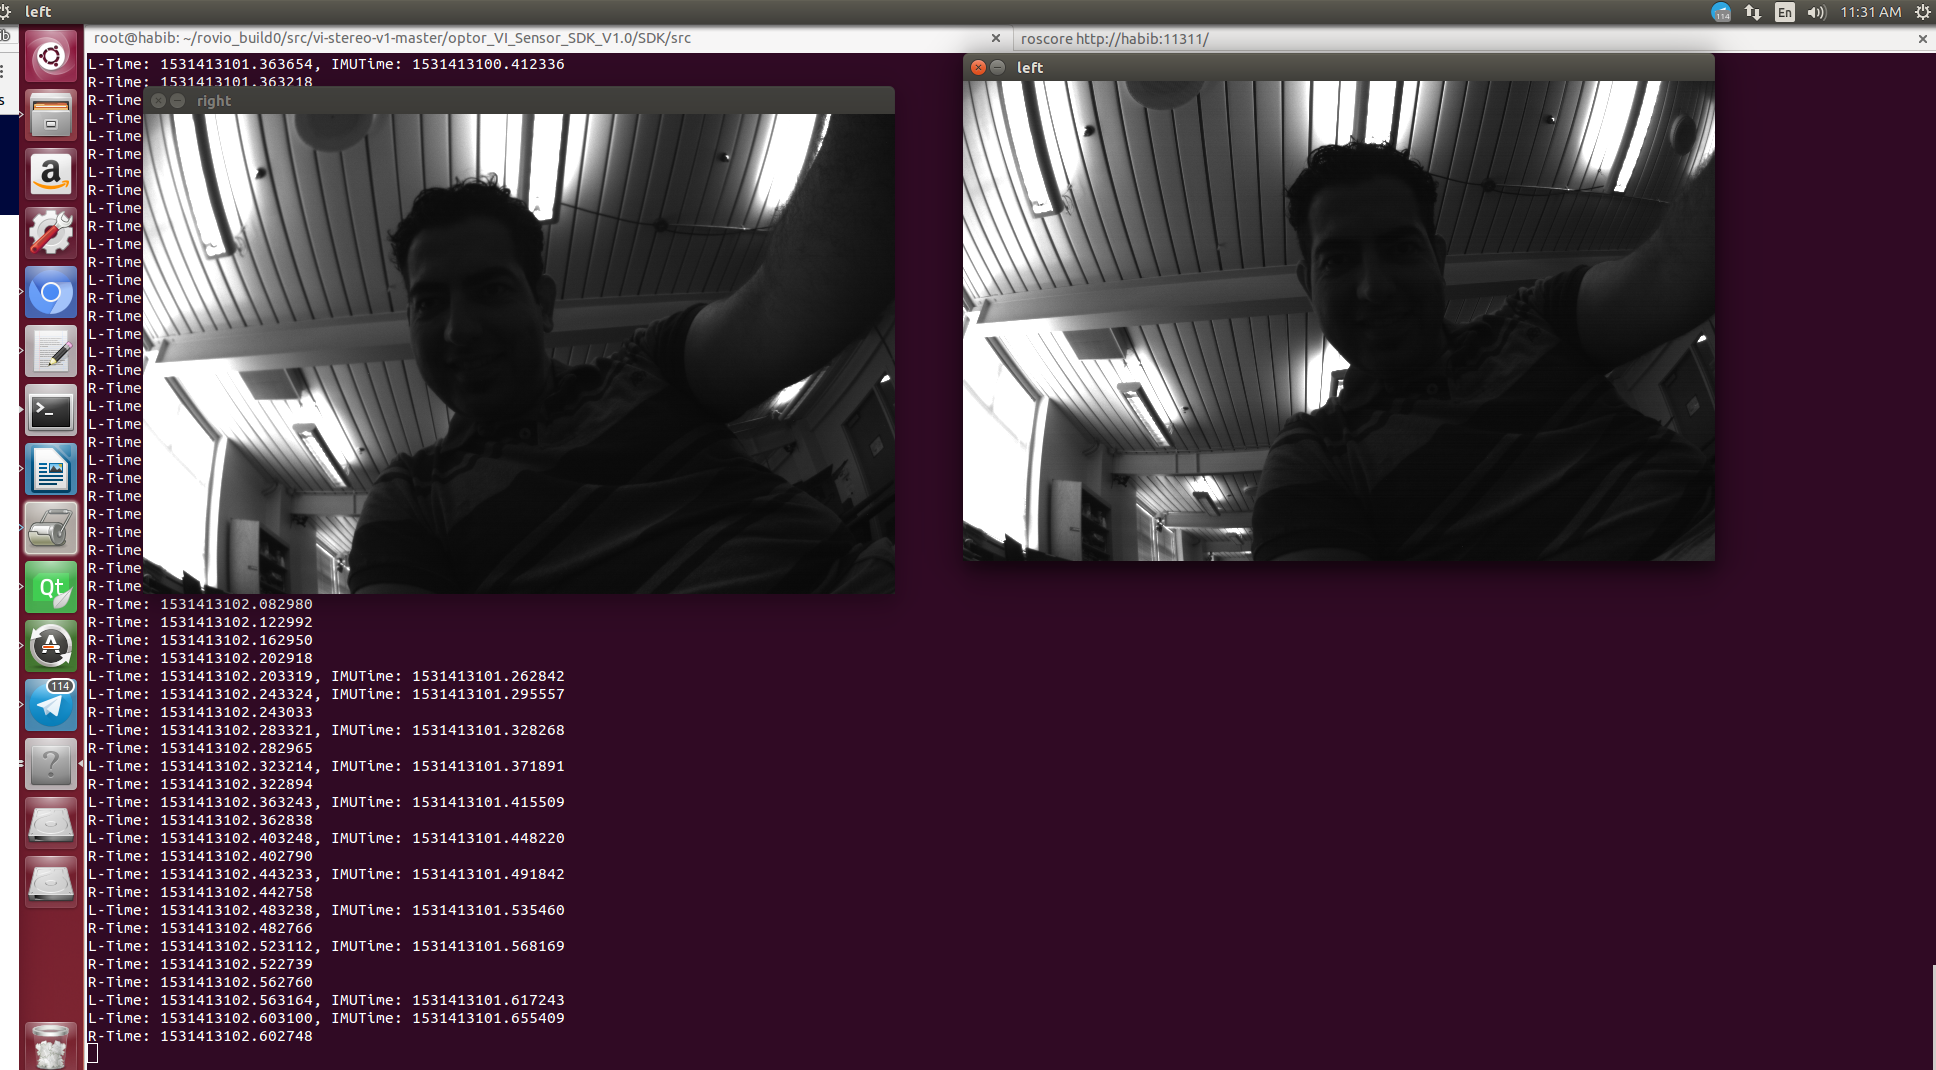
\epsfig{file =inconsistent.png, width = 5.5cm}}
  \caption{Data that received by our Visual inertial sensor.}
  \label{fig:incons}
 \end{figure}



\bibliographystyle{apalike}
{\small
\bibliography{example}}

\end{document}

